%%%%%%%%%%%%%%%%%%%%%%%%%%%%%%%%%%%%%%%%%%%%%%%%%%%%%%%%%%%%%%%%%%%%%%%%%%%%%%%%%%%%%%%%%%%%%%%%%%%%%%%%%%%%%%%%%%%%%%%%
\newpage
\chapter {\Large{Database Upgrade}}
Over time the requirement of the database within the application may change, this is almost inevitable if your application is in active development and you're constantly adding new features. Properly upgrading the database in application is important, because if something goes wrong application will have unexpected behaviour (such as crashing) or app may may loose its all data and have to start over.

\textbf{SQLite Limitation}: SQLite supports a limited subset of ALTER TABLE. The ALTER TABLE command in SQLite allows the user to rename a tablet or to add a new column to an existing table. It is not possible to rename a column, remove a column, or add or remove constraints from a table. But you can alter table column datatype or other property by the following steps:

\begin{enumerate}

	\item \small BEGIN TRANSACTION
	\item \small CREATE TEMPORARY TABLE t1\_backup(a, b);
	\item \small INSERT INTO t1\_backup SELECT a, b FROM t1;
	\item \small DROP TABLE
	\item \small CREATE TABLE t1(a, b);
	\item \small INSERT INTO t1 SELECT a, b FROM t1\_backup;
	\item \small DROP TABLE t1\_backup;
	\item \small COMMIT

\end{enumerate}

For more detail you can refer the \url{http://www.sqlite.org/lang_altertable.html}

\section{Siminov Database Upgrade}Siminov provides easy way to upgrade application database. It only support adding new table to existing database, adding a new column to existing table, and deleting existing table.

		\par
		\textbf{Example:} Siminov Template Application DatabaseDescriptor.si.xml file.
		\begin{figure}[htbp]
			\centering
				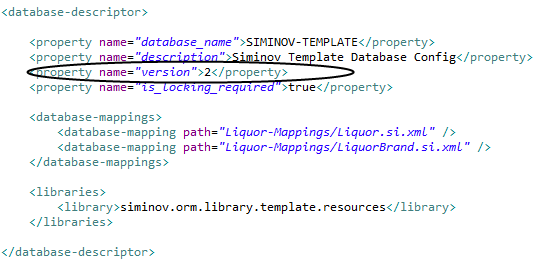
\includegraphics[height=7cm]{Resources/siminov_template_application_database_version.png}
		\end{figure}

\begin{center}
	\colorbox{grey}{
		\parbox[t]{.8\linewidth}{
			\fontsize{11pt}{11pt}\selectfont % The first argument for fontsize is the font size of the text and the second is the line spacing - you may need to play with these for your particular title
			\vspace*{0.1cm} % Space between the start of the title and the top of the grey box
		
			\hfill \textbf{Note} \\

			\hfill 	
			\begin{enumerate}
			
				\item \small Database Version should not contain decimal value.

			\end{enumerate}

			\vspace*{0.0cm} % Space between the end of the title and the bottom of the grey box
		}
	}

\end{center}
